%2_big_oh.tex
%notes for the course PandA1 COMS10002 taught at the University of Bristol
%2015 Conor Houghton conor.houghton@bristol.ac.uk

%To the extent possible under law, the author has dedicated all copyright 
%and related and neighboring rights to these notes to the public domain 
%worldwide. These notes are distributed without any warranty. 


\documentclass[11pt,a4paper]{scrartcl}
\typearea{12}
\usepackage{graphicx}
\usepackage{pstricks}
\usepackage{listings}
\usepackage{color}
\lstset{language=C}
\pagestyle{headings}
\markright{COMS10002 - PandA1 2\_big\_oh - Conor}
\begin{document}

\subsection*{2 Big Oh notation}

The \lq{}Big Oh\rq{} notation has already been used to describe the
behavior of the running time of insert sort, we said
\begin{equation}
T(n)\in O(n^2)
\end{equation}
Here we want to formalize this notation. Basically $O(n^2)$ is a set
of function, it is all the function which, for large values of $n$ go
to infinity like $n^2$ at the fastest. By saying $T(n)\in O(n^2)$ we
are saying that $T(n)$ is one of these functions, its large $n$
behavior is, at worst, like $n^2$. 

Specifically, the definition of $O(g(n)$, called \lq{}big oh\rq{} of
$g(n)$, is
\begin{equation}
O(g(n))=\{f(n)| \exists n_0>0\in {\bf N}\mbox{ and }c>0\in {\bf R}\mbox{ with }|f(n)|\le c|g(n)|\,\forall n\ge n_0\}
\end{equation}
This definition is quite dense, but we can break it down: it says that
$O(g(n))$ is a set of functions, the curly brackets mean
\lq{}set\rq{}. $f(n)$ is in the set if it has a particular
property: the \lq$|$\rq{} can be read as \lq{}such that\rq{} or
\lq{}with the property that\rq{} and so this is the set of $f(n)$'s
where $f(n)$ has the property on the right of the $|$. Now,
\lq{}$\exists$\rq{} means \lq{}there exists\rq{} and
\lq{}$\forall$\rq{} means \lq{}for all\rq{}, so the defining property
says it is possible to find a positive natural number $n_0$ and a
positive real number $c$ so that if you choose a value of $n$ at
least as big as $n_0$ then $f(n)$ is no bigger than $cg(n)$, ${\bf N}$
and ${\bf R}$ stand for the natural and real numbers. Notice the
absolute value signs, this is about $|f(n)|$ and $|g(n)|$, in fact,
here we are interested in run times, so we will deal with functions
that are non-negative, or are non-negative provided $n$ is larger than
some threshold, for example, $\log_2{n}$ will be important,
$\log_2{n}$ is positive provided $n>1$.

In short, $f(n)$ can do all sorts of crazy stuff for small values of
$n$ but, if you take $n$ large enough, its behavior is bounded by the
behavior of $g(n)$. Now it doesn't say it is bounded by $g(n)$, it is
a statement about the behavior, that's the role of the $c$. If you
know the formal definition of limits you can see that the definition
of $O(g(n))$ has this wrapped up in it, if says
\begin{equation}
f(n)\in O(g(n))\iff \lim_{n\rightarrow \infty}\frac{f(n)}{g(n)}<\infty
\end{equation}

Here are some examples, say 
\begin{equation}
T(n)=5n^2+n+6
\end{equation}
then 
\begin{equation}
T(n)\in O(n^2)
\end{equation}
by, for example, taking $c=5+1+6=12$ then 
\begin{equation}
12n^2\ge 5n^2+n+6
\end{equation}
provided $n\ge 1$ so $n_0=1$ here. This could also be succinctly
demonstrated using the limit
\begin{equation}
\lim_{n\rightarrow \infty} \frac{5n^2+n+6}{n^2}=\lim_{n\rightarrow \infty}5+\lim_{n\rightarrow \infty}\frac{1}{n}+\lim_{n\rightarrow \infty}\frac{6}{n^2}=5<\infty
\end{equation}

However, 
\begin{equation}
T(n)\not\in O(n)
\end{equation}
Say we chosen some value $c$ then
\begin{equation}
5n^2+n+6>cn
\end{equation}
for large enough $n$, to check this divide both sides by $n$ so we need to show that $n$ can be chosen so that
\begin{equation}
5n+1+\frac{c}{n}>c
\end{equation}
Since 
\begin{equation}
5n+1+\frac{c}{n}>5n+1
\end{equation}
then, if $n>c/5$
\begin{equation}
5n+1+\frac{c}{n}>5\frac{c}{5}+1=c+1>c
\end{equation}
so, no matter what value of $c$ is chosen, making $n>5/n$ implies
\begin{equation}
5n^2+n+6>cn
\end{equation}
so $5n^2+n+6\not\in O(n)$. Again, the limit does the same job
\begin{equation}
\lim_{n\rightarrow \infty} \frac{5n^2+n+6}{n}=\lim_{n\rightarrow \infty}5n+\lim_{n\rightarrow \infty}1+\lim_{n\rightarrow \infty}\frac{6}{n}=\infty
\end{equation}


In practice, if
\begin{equation}
T(n)=a_rn^r+a_{r-1}n^{r-1}+\ldots+a_1n+a_0
\end{equation}
then $T(n)\in O(n^r)$. 

The logarithm has the funny property that it goes to infinity, but it
does so slower than $n$:
\begin{equation}
\lim_{n\rightarrow \infty}\frac{\log_2{n}}{n}=0
\end{equation}
Here, in line with standard practice in computer science, we are using
the log to the base two, in fact changing bases only causes a change
of an overall constant, see Table~\ref{math_logs} for a reminder of
the properties of the log. The limit of $\log_2{n}/n$ can be
calculated using l'H\^{o}pital's rule, here we'll just look at a plot,
Fig.~\ref{fig_log}. Now, just as $\log_2{n}$ grows very slowly, $2^n$
grows very fast,
\begin{equation}
\lim_{n\rightarrow \infty}\frac{n^r}{2^n}=0
\end{equation}
for any finite value of $r$, worse still is $n!$, pronounced $n$-factorial
\begin{equation}
n!=n(n-1)(n-2) . . . 1
\end{equation}
If your algorithm is in $O(n!)$ you will probably need a different
algorithm. A table of different values is given as
Table~\ref{table_n_values}, mostly to emphasis how quickly $n!$ gets
big.

Now, in mathematics we call something \lq{}an abuse of notation\rq{}
if it is common to write something that doesn't quite make sense but
acts as a shorthand for something that does. Now $O(g(n))$ is a set of
functions whose large $n$ behavior is bounded by $g(n)$ so in
algorithms, being in $O(g(n))$ is a property of $T(n)$, the formula
for the running time of the algorithm. However, it is a standard abuse
of notation to say an algorithm is $O(g(n))$ for some $g(n)$ is
$T(n)\in O(g(n))$ for all cases. This is another way of saying that
the worst behavior of the algorithm isn't any worse than the behavior
of $g(n)$ for large $n$ so all possible $T(n)$ are elements of
$O(g(n))$.

\begin{table}
\color{darkgray}
The logarithm is the opposite of the exponent: if
\begin{equation}
a^b=c
\end{equation}
then 
\begin{equation}
\log_a{c}=b
\end{equation}
or, written in one line
\begin{equation}
a^{\log_a{c}}=c
\end{equation}
All the laws of logs can be worked out from the laws of
exponents. Hence, since $a^0=1$ we have $\log_a{1}=0$. In a similar
way, other rules of logs can be deduced like
\begin{eqnarray}
\log_a{c_1c_2}&=&\log_a{c_1}+\log_a{c_2}\cr
\log_a{\frac{c_1}{c_2}}&=&\log_a{c_1}-\log_a{c_2}\cr
\log_a c^d&=&d\log_a c
\end{eqnarray}
and so on.

As for the change of base, let $b=\log_{a_1}{c}$ so $a_1^{b}=c$. Now take the log to the base $a_2$ of both sides
\begin{equation}
b\log_{a_2}a_1=\log_{a_2}{c}
\end{equation}
and then solve for $b$
\begin{equation}
b=\frac{\log_{a_2}c}{\log_{a_2}a_1}
\end{equation}
and, substituting back the formula for $b$
\begin{equation}
\log_{a_1}{c}=\frac{\log_{a_2}c}{\log_{a_2}a_1}
\end{equation}
Thus we see, that changing bases is just a matter of a
multiplicative factor. For example, to change from base $e$ to base two
\begin{equation}
\log_{2}{x}=\frac{\log_e{x}}{\log_e{2}}\approx\frac{\log_e{x}}{0.6931}
\end{equation}
Common bases are $\log_2{x}$ used in computer science, $\log_e{x}$
sometimes written $\ln{x}$ used in mathematics and $\log_{10}{x}$ used
in chemistry. The base two is used because of its link to bits and
also, as we will see, because of its relationship with algorithms that
divide data into two piles. The natural log $\ln{x}$ is used where
differential equations are common since
\begin{equation}
\frac{d}{dx}\ln{x}=\frac{1}{x}
\end{equation}
\caption{A reminder about logarithms. This is a quick summary of some of the laws of logs.\label{math_logs}}
\color{black}
\end{table}

\begin{figure}
% GNUPLOT: LaTeX picture with Postscript
\begingroup
  \makeatletter
  \providecommand\color[2][]{%
    \GenericError{(gnuplot) \space\space\space\@spaces}{%
      Package color not loaded in conjunction with
      terminal option `colourtext'%
    }{See the gnuplot documentation for explanation.%
    }{Either use 'blacktext' in gnuplot or load the package
      color.sty in LaTeX.}%
    \renewcommand\color[2][]{}%
  }%
  \providecommand\includegraphics[2][]{%
    \GenericError{(gnuplot) \space\space\space\@spaces}{%
      Package graphicx or graphics not loaded%
    }{See the gnuplot documentation for explanation.%
    }{The gnuplot epslatex terminal needs graphicx.sty or graphics.sty.}%
    \renewcommand\includegraphics[2][]{}%
  }%
  \providecommand\rotatebox[2]{#2}%
  \@ifundefined{ifGPcolor}{%
    \newif\ifGPcolor
    \GPcolorfalse
  }{}%
  \@ifundefined{ifGPblacktext}{%
    \newif\ifGPblacktext
    \GPblacktexttrue
  }{}%
  % define a \g@addto@macro without @ in the name:
  \let\gplgaddtomacro\g@addto@macro
  % define empty templates for all commands taking text:
  \gdef\gplbacktext{}%
  \gdef\gplfronttext{}%
  \makeatother
  \ifGPblacktext
    % no textcolor at all
    \def\colorrgb#1{}%
    \def\colorgray#1{}%
  \else
    % gray or color?
    \ifGPcolor
      \def\colorrgb#1{\color[rgb]{#1}}%
      \def\colorgray#1{\color[gray]{#1}}%
      \expandafter\def\csname LTw\endcsname{\color{white}}%
      \expandafter\def\csname LTb\endcsname{\color{black}}%
      \expandafter\def\csname LTa\endcsname{\color{black}}%
      \expandafter\def\csname LT0\endcsname{\color[rgb]{1,0,0}}%
      \expandafter\def\csname LT1\endcsname{\color[rgb]{0,1,0}}%
      \expandafter\def\csname LT2\endcsname{\color[rgb]{0,0,1}}%
      \expandafter\def\csname LT3\endcsname{\color[rgb]{1,0,1}}%
      \expandafter\def\csname LT4\endcsname{\color[rgb]{0,1,1}}%
      \expandafter\def\csname LT5\endcsname{\color[rgb]{1,1,0}}%
      \expandafter\def\csname LT6\endcsname{\color[rgb]{0,0,0}}%
      \expandafter\def\csname LT7\endcsname{\color[rgb]{1,0.3,0}}%
      \expandafter\def\csname LT8\endcsname{\color[rgb]{0.5,0.5,0.5}}%
    \else
      % gray
      \def\colorrgb#1{\color{black}}%
      \def\colorgray#1{\color[gray]{#1}}%
      \expandafter\def\csname LTw\endcsname{\color{white}}%
      \expandafter\def\csname LTb\endcsname{\color{black}}%
      \expandafter\def\csname LTa\endcsname{\color{black}}%
      \expandafter\def\csname LT0\endcsname{\color{black}}%
      \expandafter\def\csname LT1\endcsname{\color{black}}%
      \expandafter\def\csname LT2\endcsname{\color{black}}%
      \expandafter\def\csname LT3\endcsname{\color{black}}%
      \expandafter\def\csname LT4\endcsname{\color{black}}%
      \expandafter\def\csname LT5\endcsname{\color{black}}%
      \expandafter\def\csname LT6\endcsname{\color{black}}%
      \expandafter\def\csname LT7\endcsname{\color{black}}%
      \expandafter\def\csname LT8\endcsname{\color{black}}%
    \fi
  \fi
  \setlength{\unitlength}{0.0500bp}%
  \begin{picture}(7200.00,5040.00)%
    \gplgaddtomacro\gplbacktext{%
      \csname LTb\endcsname%
      \put(726,704){\makebox(0,0)[r]{\strut{} 0}}%
      \put(726,1383){\makebox(0,0)[r]{\strut{} 0.5}}%
      \put(726,2061){\makebox(0,0)[r]{\strut{} 1}}%
      \put(726,2740){\makebox(0,0)[r]{\strut{} 1.5}}%
      \put(726,3418){\makebox(0,0)[r]{\strut{} 2}}%
      \put(726,4097){\makebox(0,0)[r]{\strut{} 2.5}}%
      \put(726,4775){\makebox(0,0)[r]{\strut{} 3}}%
      \put(858,484){\makebox(0,0){\strut{} 1}}%
      \put(1849,484){\makebox(0,0){\strut{} 1.5}}%
      \put(2840,484){\makebox(0,0){\strut{} 2}}%
      \put(3831,484){\makebox(0,0){\strut{} 2.5}}%
      \put(4821,484){\makebox(0,0){\strut{} 3}}%
      \put(5812,484){\makebox(0,0){\strut{} 3.5}}%
      \put(6803,484){\makebox(0,0){\strut{} 4}}%
      \put(3830,154){\makebox(0,0){\strut{}$x$}}%
    }%
    \gplgaddtomacro\gplfronttext{%
      \csname LTb\endcsname%
      \put(1450,4602){\makebox(0,0)[r]{\strut{}$\log_2{x}$}}%
      \csname LTb\endcsname%
      \put(1450,4382){\makebox(0,0)[r]{\strut{}$x-1$}}%
    }%
    \gplbacktext
    \put(0,0){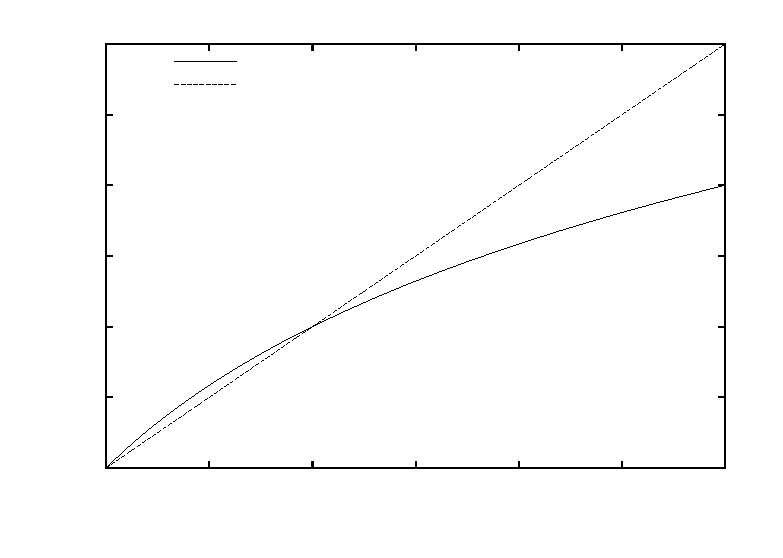
\includegraphics{I.2.log.eps}}%
    \gplfronttext
  \end{picture}%
\endgroup

\caption{This shows $\log_2{x}$ and $x-1$ plots for $x\in[1,4]$, the one has been taken from $x$ to make them easier to compare, the key point is that the $x$ grows faster.\label{fig_log}}
\end{figure}


\begin{figure}
% GNUPLOT: LaTeX picture with Postscript
\begingroup
  \makeatletter
  \providecommand\color[2][]{%
    \GenericError{(gnuplot) \space\space\space\@spaces}{%
      Package color not loaded in conjunction with
      terminal option `colourtext'%
    }{See the gnuplot documentation for explanation.%
    }{Either use 'blacktext' in gnuplot or load the package
      color.sty in LaTeX.}%
    \renewcommand\color[2][]{}%
  }%
  \providecommand\includegraphics[2][]{%
    \GenericError{(gnuplot) \space\space\space\@spaces}{%
      Package graphicx or graphics not loaded%
    }{See the gnuplot documentation for explanation.%
    }{The gnuplot epslatex terminal needs graphicx.sty or graphics.sty.}%
    \renewcommand\includegraphics[2][]{}%
  }%
  \providecommand\rotatebox[2]{#2}%
  \@ifundefined{ifGPcolor}{%
    \newif\ifGPcolor
    \GPcolorfalse
  }{}%
  \@ifundefined{ifGPblacktext}{%
    \newif\ifGPblacktext
    \GPblacktexttrue
  }{}%
  % define a \g@addto@macro without @ in the name:
  \let\gplgaddtomacro\g@addto@macro
  % define empty templates for all commands taking text:
  \gdef\gplbacktext{}%
  \gdef\gplfronttext{}%
  \makeatother
  \ifGPblacktext
    % no textcolor at all
    \def\colorrgb#1{}%
    \def\colorgray#1{}%
  \else
    % gray or color?
    \ifGPcolor
      \def\colorrgb#1{\color[rgb]{#1}}%
      \def\colorgray#1{\color[gray]{#1}}%
      \expandafter\def\csname LTw\endcsname{\color{white}}%
      \expandafter\def\csname LTb\endcsname{\color{black}}%
      \expandafter\def\csname LTa\endcsname{\color{black}}%
      \expandafter\def\csname LT0\endcsname{\color[rgb]{1,0,0}}%
      \expandafter\def\csname LT1\endcsname{\color[rgb]{0,1,0}}%
      \expandafter\def\csname LT2\endcsname{\color[rgb]{0,0,1}}%
      \expandafter\def\csname LT3\endcsname{\color[rgb]{1,0,1}}%
      \expandafter\def\csname LT4\endcsname{\color[rgb]{0,1,1}}%
      \expandafter\def\csname LT5\endcsname{\color[rgb]{1,1,0}}%
      \expandafter\def\csname LT6\endcsname{\color[rgb]{0,0,0}}%
      \expandafter\def\csname LT7\endcsname{\color[rgb]{1,0.3,0}}%
      \expandafter\def\csname LT8\endcsname{\color[rgb]{0.5,0.5,0.5}}%
    \else
      % gray
      \def\colorrgb#1{\color{black}}%
      \def\colorgray#1{\color[gray]{#1}}%
      \expandafter\def\csname LTw\endcsname{\color{white}}%
      \expandafter\def\csname LTb\endcsname{\color{black}}%
      \expandafter\def\csname LTa\endcsname{\color{black}}%
      \expandafter\def\csname LT0\endcsname{\color{black}}%
      \expandafter\def\csname LT1\endcsname{\color{black}}%
      \expandafter\def\csname LT2\endcsname{\color{black}}%
      \expandafter\def\csname LT3\endcsname{\color{black}}%
      \expandafter\def\csname LT4\endcsname{\color{black}}%
      \expandafter\def\csname LT5\endcsname{\color{black}}%
      \expandafter\def\csname LT6\endcsname{\color{black}}%
      \expandafter\def\csname LT7\endcsname{\color{black}}%
      \expandafter\def\csname LT8\endcsname{\color{black}}%
    \fi
  \fi
  \setlength{\unitlength}{0.0500bp}%
  \begin{picture}(7200.00,5040.00)%
    \gplgaddtomacro\gplbacktext{%
      \csname LTb\endcsname%
      \put(594,440){\makebox(0,0)[r]{\strut{} 0}}%
      \put(594,1059){\makebox(0,0)[r]{\strut{} 10}}%
      \put(594,1679){\makebox(0,0)[r]{\strut{} 20}}%
      \put(594,2298){\makebox(0,0)[r]{\strut{} 30}}%
      \put(594,2917){\makebox(0,0)[r]{\strut{} 40}}%
      \put(594,3536){\makebox(0,0)[r]{\strut{} 50}}%
      \put(594,4156){\makebox(0,0)[r]{\strut{} 60}}%
      \put(594,4775){\makebox(0,0)[r]{\strut{} 70}}%
      \put(726,220){\makebox(0,0){\strut{} 0}}%
      \put(1739,220){\makebox(0,0){\strut{} 1}}%
      \put(2752,220){\makebox(0,0){\strut{} 2}}%
      \put(3765,220){\makebox(0,0){\strut{} 3}}%
      \put(4777,220){\makebox(0,0){\strut{} 4}}%
      \put(5790,220){\makebox(0,0){\strut{} 5}}%
      \put(6803,220){\makebox(0,0){\strut{} 6}}%
    }%
    \gplgaddtomacro\gplfronttext{%
      \csname LTb\endcsname%
      \put(5816,4602){\makebox(0,0)[r]{\strut{}$2^x$}}%
      \csname LTb\endcsname%
      \put(5816,4382){\makebox(0,0)[r]{\strut{}$x^2+1$}}%
    }%
    \gplbacktext
    \put(0,0){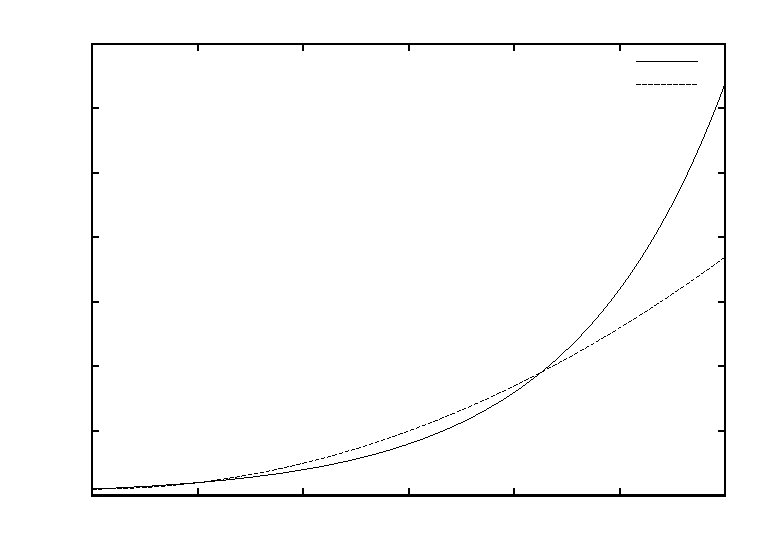
\includegraphics{exp.eps}}%
    \gplfronttext
  \end{picture}%
\endgroup

\caption{This shows $2^x$ and $x^2-1$ plots for $x\in[0,6]$, clearly $2^x$ quickly overtakes $x^2+1$, this will happen for any power of $x$. \label{fig_log}}
\end{figure}

\begin{table}
\begin{tabular}{l|cccccc}
        $n$    &1   &2&4   &16  &128&1024\\
$\log{n}$      &0   &1&2   &4   &7  &10\\
$n\log{n}$     &0   &2&8   &64  &896&10240\\
$n^2$     &1   &4&16&256&16384&1048576\\
$2^n$     &2   &4&16&65536&$3.4\times 10^{38}$&$1.8\times 10^{307}$\\
$n!$      &1   &2&24&$2.1\times 10^{13}$&$3.85\times 10^{305}$&$5.4\times10^{2369}$
\end{tabular}
\vskip 1cm The website\\ {\tt
  http://markknowsnothing.com/cgi-bin/calculator.php}\\ was used for
the $2^n$ calculations and\\ {\tt
  http://www.calculatorsoup.com/calculators/discretemathematics/factorials.php}\\ for
the $n!$ calculations; these give answers even when the answer is very
large. Another easy way to calculate with large numbers is to use Python.

\caption{Different values of $n$ for some functions.  \label{table_n_values}
}
\end{table}

\subsubsection*{Other big Letter notations, small oh notation.}

There is another set, $\Omega(g(n))$ with a definition similar to
$O(g(n))$ that is used for describing the best case behavior. This
requires a lower bound rather than an upper bound, so the obvious
definition is
\begin{equation}
\Omega(g(n))=\{f(n)| \exists n_0>0\in {\bf N}\mbox{ and }c>0\in {\bf R}\mbox{ with }|f(n)|\ge c|g(n)|\,\forall n\ge n_0\}
\end{equation}
in other words, the same thing, but with the $\le$ symbol replaced by
a $\ge$. In fact, there is some ambiguity about this definition,
number theorist use a slightly different one. Either way, it isn't
used very often in computer science because algorithms are very
frequently $\Omega(1)$; in the best case scenario the problem is in
some sense already solve, the array already sorted for example, and
the algorithm finishs in one step. 

There is also a set of function that are both bounded above and below
by the same $g(n)$
\begin{equation}
\Theta(g(n))=\Omega(g(n))\cap O(g(n))
\end{equation}
This works because it is possible for
\begin{equation}
c_1 g(n)\le f(n)\le c_2g(n)
\end{equation}
for different $c_1$ and $c_2$. It would be very unusual for this to
apply to an algorithm, it would mean that $T(n)$ has the same behavior
for large $n$ no matter whether it is the best case or the worst case
scenario. There is a na\"ive largest element function in
Table~\ref{c_largest_linear_search} which is $\Theta(n)$. It searches
for the largest value in an unsorted array by looking at each element
in turn. In fact, for a completely unsorted array this is the best
algorithm, but, in practice, if finding the largest element in a set
is an important and frequent procedure, a special data structure,
called a heap, is used to keep track of which element is largest.

\begin{table}
\begin{lstlisting}[numbers=left]
int search(int a[],int n)
{
   int i;
   int best_val=a[0];

   for(i=1;i<n;i++){
      if(a[i]>best_val)
         best_val= a[i];
   }

  return best_val;
}
\end{lstlisting}
\caption{Search for the largest element in an unsorted list. This
  function searches all the elements to see which is the largest, the
  inner loop always runs $n-1$ times since it doesn't know until it
  has looked at every element which is going to be the largest. This
  program is implemented as {\tt
    find\_largest.c}.\label{c_largest_linear_search}.}
\end{table}

Finally, little oh notation is a stricter version of big Oh notation
that is used in some more mathematical context, basically $f(n)\in
o(g(n))$ is $f(n)$ is less than $cg(n)$ for any choice of $c$, if $n$
is large enough:
\begin{equation}
\o(g(n))=\{f(n)| \exists n_0>0\in {\bf N}\mbox{ so that }|f(n)|\ge
c|g(n)|\,\forall n\ge n_0 \mbox{ and }\forall\,c>0\in {\bf R}\}
\end{equation}

\end{document}
